\documentclass{report}
\usepackage{float}

% depricated
\title{
	\iffalse
	\begin{tikzpicture}[remember picture,overlay]
		\node[anchor=north west,yshift=-5pt,xshift=-200pt]%
		at (current page.north east)
		{
\includegraphics[height=30mm]{unitn-logo}};
	\end{tikzpicture}
	\huge 
	\fi
	Fix Mi \\
	Analisi dei Requisiti
}
\author{Giovanni Santini, Riginel Ungureanu, Valerio Asaro}
\date{Anno accademico 2023/2024}

% for the image in the title
\usepackage{tikz}

% custom spacing
\usepackage{setspace}
\onehalfspacing

% footer and header
\usepackage{fancyhdr}
% \setlength{\headheight}{15.2pt}

% underlining
\usepackage{ulem}


% Table of contents link to corresponding sections
\usepackage{hyperref}
\hypersetup{
	colorlinks,
	citecolor=black,
	filecolor=black,
	linkcolor=black,
	urlcolor=black
}

\usepackage{amsmath}
% Remove che "Chapter" string before chapters
\iffalse
\makeatletter
\def\@makechapterhead#1{%
	\vspace*{50\p@}%
	{\parindent \z@ \raggedright \normalfont
		\interlinepenalty\@M
		\Huge\bfseries  \thechapter.\quad #1\par\nobreak
		\vskip 40\p@
}}
\makeatother
\fi

% Fancy chapters
\usepackage[Bjarne]{fncychap}
% options: Sonny, Lenny, Glenn, Conny, Rejne, Bjarne, Bjornstrup

\begin{document}
	
	
	%title page
	\begin{titlepage}
		\begin{figure}[t]
			\centering
\includegraphics[width=0.3\textwidth]{images/unitn-logo}
		\end{figure}
		\begin{center}
			\textsc{ \LARGE{Università degli Studi di Trento \\}}
			\textsc{ \LARGE{Facoltà di Informatica\\ }}
			\textnormal{ \LARGE{Corso di Ingegneria del Software\\}}
			\vspace{30mm}
			\fontsize{10mm}{7mm}\selectfont 
			\textup{Fix Mi \\ Specifica dei Requisiti}\\
		\end{center}
		
		\vspace{25mm}
		
		\centering
		\large Gruppo G43: \\ Giovanni Santini\\ Riginel Ungureanu \\ Valerio Asaro
		
		\vspace{20mm}
		
		\centering{\large{Anno Accademico 2023/2024 \\ Trento }}
		
	\end{titlepage}
	
	
	
	
	% use header and footers
	\pagestyle{fancy}
	\fancyhead[R]{\chaptername\ \thechapter}  % header
	
	%\maketitle
	\tableofcontents
	\newpage
	
	
	
	\section{Scopo del documento}
	
	Nel presente documento vengono riportate le specifiche dei requisiti di sistema del progetto FixMi,  attraverso diagrammi di tipo Unified Modeling Language (UML) e tabelle strutturate.\\
	
	
	
	\section{Informazioni del Documento}
	
	% table
	\begin{center} % center the table
		\centering
		\begin{tabular}{ |p{4cm}|p{4cm}|  }
			\hline
			\centering Campo & \qquad\qquad Valore \\ % I found no other way...
			\hline
			Titolo del Documento & Specifica dei Requisiti \\
			\hline
			Titolo del Progetto & Fix Mi \\
			\hline
			Autori del Documento &
			Giovanni Santini \\ & Riginel Ungureanu \\ & Valerio Asaro \\
			\hline
			Amministratore Progetto & Riginel Ungureanu\\
			\hline
			Versione del documento & 1.0 \\
			\hline
		\end{tabular}
	\end{center}


\chapter{Requisiti}

	
\section{Requisiti Funzionali}

\begin{itemize}
	\item Use Case Diagram: Visione esterna del sistema
	\item Sequence Diagram: Rappresenta come gli oggetti collaborano
	\item State Machine Diagram: Stati e Transizioni
	\item Activity Diagram: Attività che innescano altre attività (tasks)
	\item Spiegazione in italiano (da mettere sempre)
\end{itemize}

\subsection*{RF1 Login }
\begin{figure}[H]
	\centering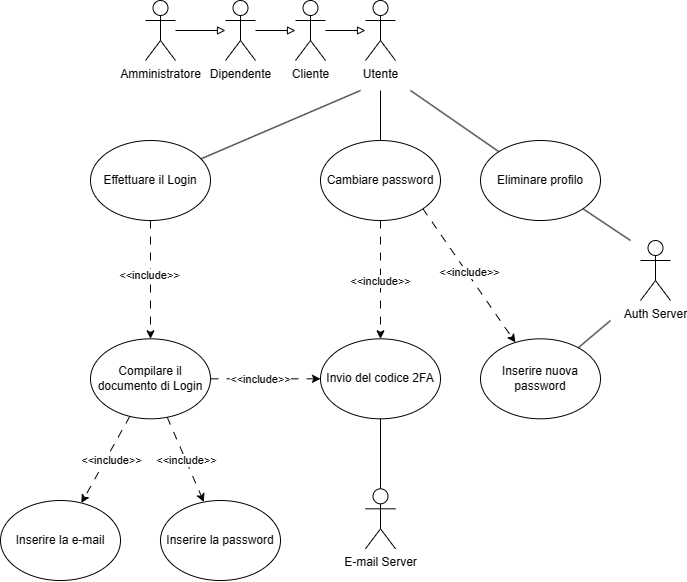
\includegraphics[width=1\textwidth]{images/UCD/RF1_login_UCD.png}
	Use Case Diagram (UCD) di RF1 "Login"
\end{figure}
Per descrivere questo use case, facciamo uso di due diagrammi delle attività swimlane:
\begin{figure}[H]
	\centering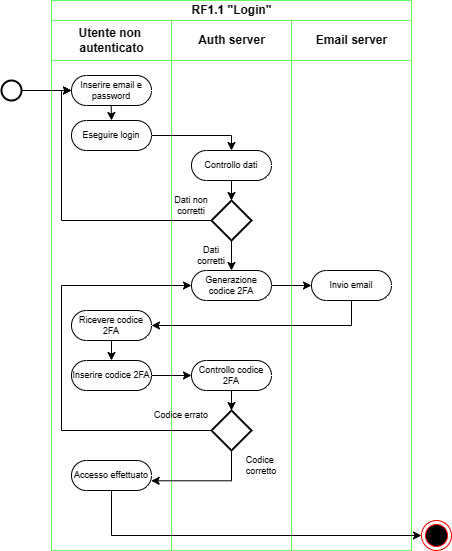
\includegraphics[width=1\textwidth]{images/Login_Swimlane.drawio.png}
	diagramma delle Attività swimlane del Login
\end{figure}
\begin{figure}[H]
	\centering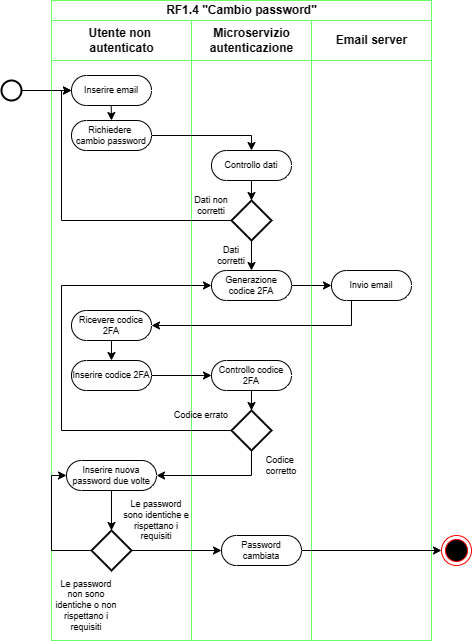
\includegraphics[width=1\textwidth]{images/password_change_swimlane.drawio.png}
	diagramma delle Attività swimlane del cambio password
\end{figure}
\subsection*{RF2 Registrazione}
\begin{figure}[H]
	\centering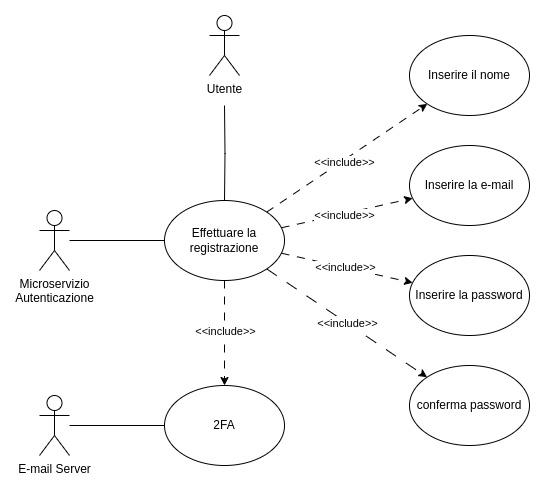
\includegraphics[width=1\textwidth]{images/UCD/RF2_registrazione_UCD.png}
	Use Case Diagram (UCD) di RF2 "Registrazione"
\end{figure}
Per descrivere questo use case, facciamo uso di un diagramma delle attività swimlane:
\begin{figure}[H]
	\centering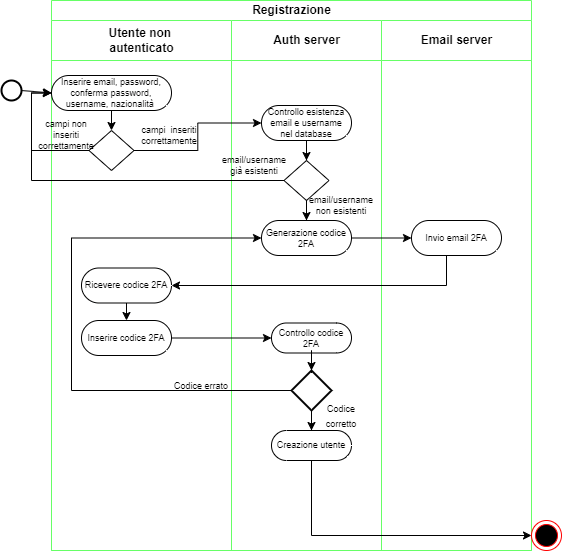
\includegraphics[width=1\textwidth]{images/Register_swimlane.drawio.png}
	diagramma delle Attività swimlane della registrazione
\end{figure}

\subsection*{RF4 Informazioni / Contatti}

\textbf{Titolo}: Informazioni / Contatti\\
\textbf{Descrizione}: L'utente cliccando la pagina "Informazioni / Contatti" visualizza le informazioni e i contatti dell'azienda, quali una descrizione, l'indirizzo e la posizione nella mappa, contatti telefonici, e-amil e FAQ.

\begin{figure}[H]
	\centering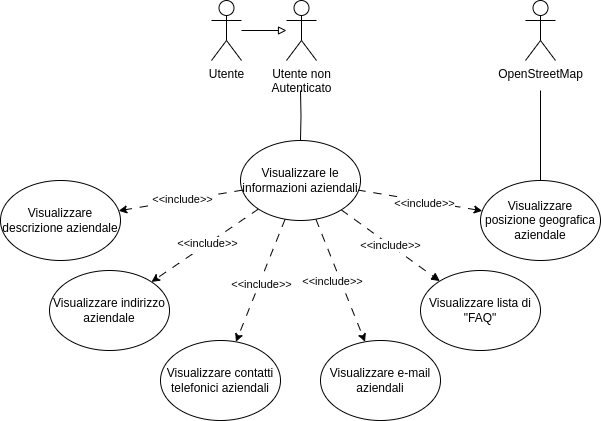
\includegraphics[width=1\textwidth]{images/UCD/RF4_infocontatti_UCD.png}
	Use Case Diagram (UCD) di RF4 "Informazioni / Contatti"
\end{figure}


\subsection*{RF3 Negozio Utente e RF5 Negozio Cliente}

\begin{figure}[H]
	\centering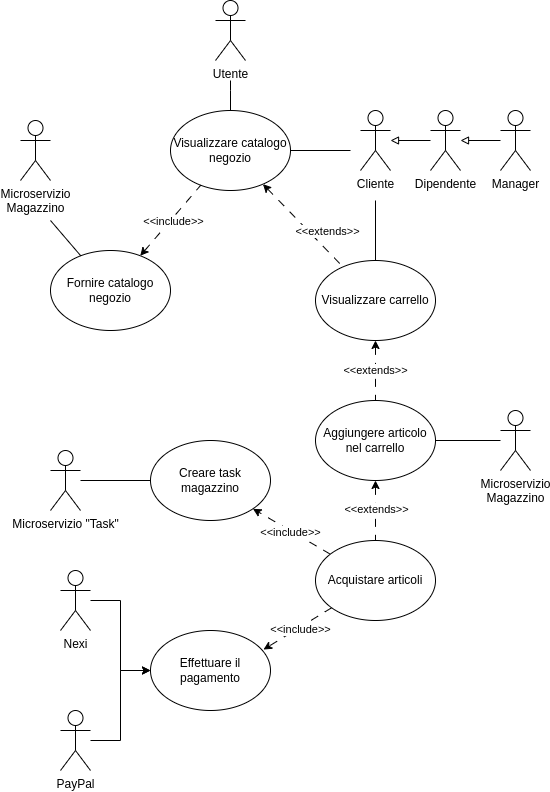
\includegraphics[width=1\textwidth]{images/UCD/RF3+5_negozio_UCD.png}
	Use Case Diagram (UCD) di RF3 e RF5 "Negozio"
\end{figure}

\begin{figure}[H]
	\centering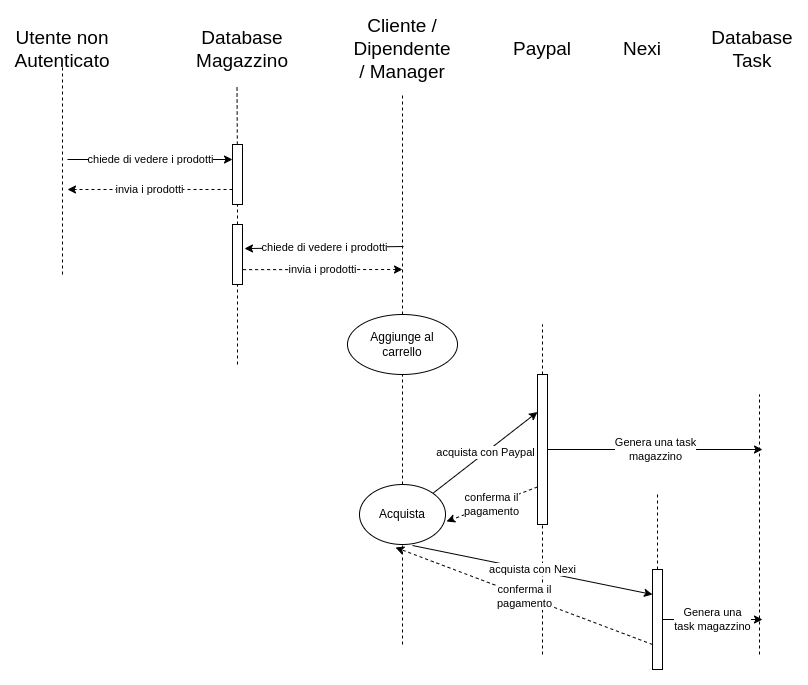
\includegraphics[width=1\textwidth]{images/negozio_sequence_diagram.png}
	diagramma delle Attività swimlane della registrazione
\end{figure}

\subsection*{RF6 Riparazione}
\begin{figure}[H]
	\centering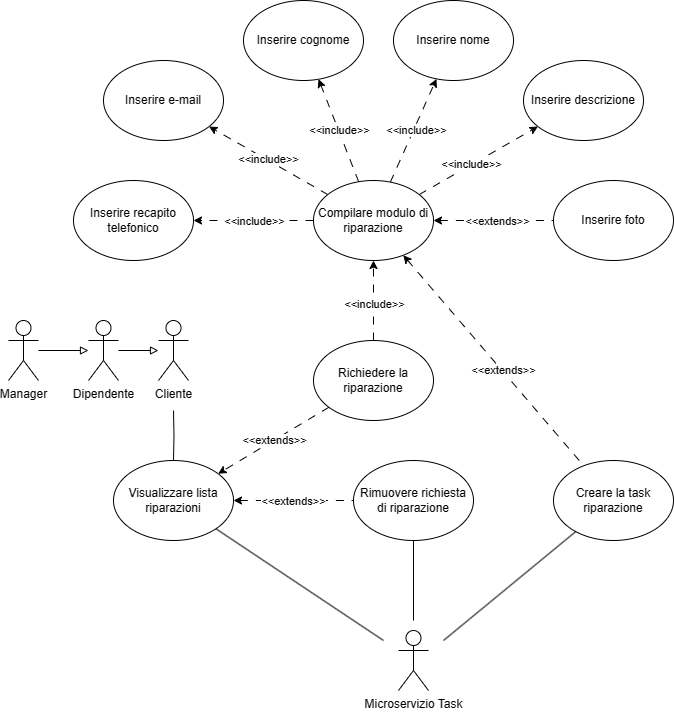
\includegraphics[width=1\textwidth]{images/UCD/RF6_riparazione_UCD.png}
	Use Case Diagram (UCD) di RF6 "Riparazione"
\end{figure}
\subsubsection*{Descrizione Use Case "Riparazione"}
\textbf{Titolo}: Riparazione \newline
\textbf{Riassunto}: Questo use case descrive come un utente può richiedere una riparazione e visualizzarne lo stato. \newline
\textbf{Descrizione}:
	\begin{enumerate}
		\item L'utente autenticato seleziona la pagina "Riparazioni";
		\item Il sito mostra lo stato delle riparazioni già richieste dall'utente [Exception 1];
		\item Il sito mostra un form per richiedere una nuova riparazione con i seguenti campi:
		\begin{itemize}
			\item nome[Exception 2];
			\item cognome[Exception 2]; 
			\item e-mail[Exception 2];
			\item numero di telefono[Exception 2];
			\item descrizione del problema[Exception 2];
			\item foto (( facoltativo ));
		\end{itemize}
		\item L'utente, appena compilato il form, può inviarlo premendo l'apposito pulsante;
		\item Il sistema, appena ricevuta la richiesta d.i riparazione, la inserisce nel sistema delle task come "task riparazione";
		
	\end{enumerate}
\textbf{Exceptions}
\begin{itemize}
	\item {[Exception 1]}: Se L'utente non ha nessuna riparazione richiesta, l'elenco sarà vuoto;
	\item {[Exception 2]}: Se l'utente non ha compilato i campi "nome","cognome","e-mail","numero di telefono","descrizione del problema" non può inviare la richiesta;
\end{itemize}
\subsection*{RF7 Assistenza}

\begin{figure}[H]
	\centering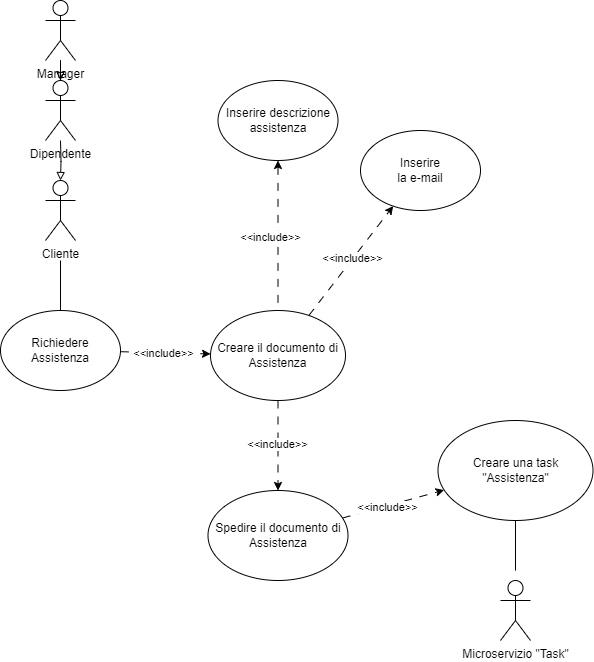
\includegraphics[width=1\textwidth]{images/UCD/RF7_assistenza_UCD.png}
	Use Case Diagram (UCD) di RF7 "Assistenza"
\end{figure}


\subsection*{RF8 Feedback}

\begin{figure}[H]
	\centering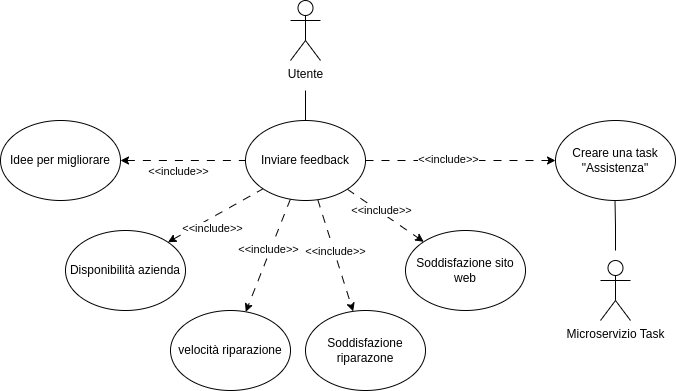
\includegraphics[width=1\textwidth]{images/UCD/RF8_feedback_UCD.png}
	Use Case Diagram (UCD) di RF8 "Feedback"
\end{figure}

\subsection*{RF9 Tasks}

\begin{figure}[H]
	\centering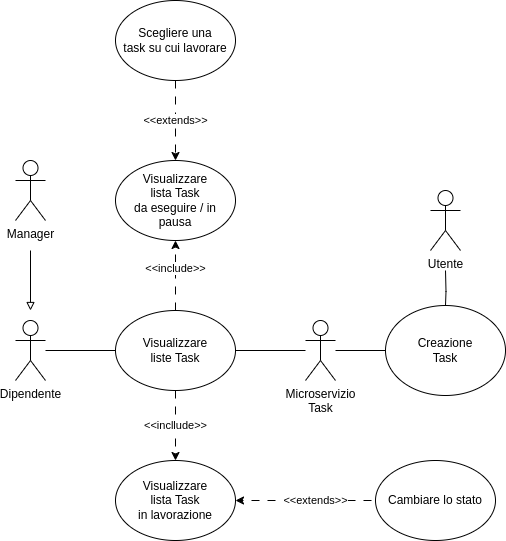
\includegraphics[width=1\textwidth]{images/UCD/RF9_task_UCD.png}
	Use Case Diagram (UCD) di RF9 "Task"
\end{figure}

Descrizione a parola qua

\begin{figure}[H]
	\centering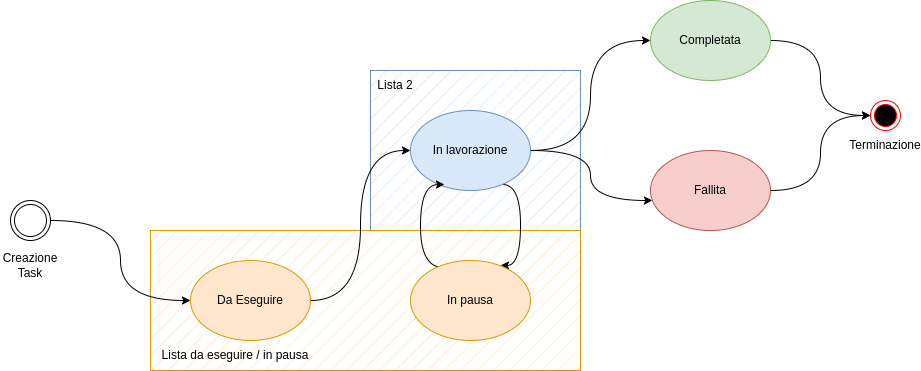
\includegraphics[width=1\textwidth]{images/state_diagram_task.png}
	State Diagram di RF9 "Task"
\end{figure}

\subsection*{RF10 Magazzino}
\begin{figure}[H]
	\centering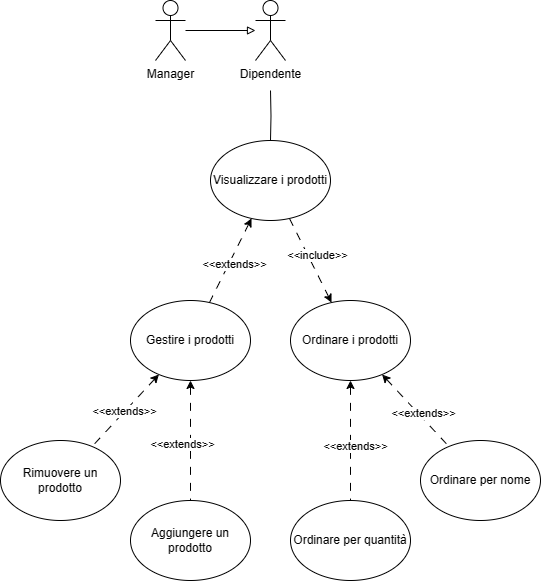
\includegraphics[width=1\textwidth]{images/UCD/RF10_magazzino_UCD.png}
	Use Case Diagram (UCD) di RF10 "Magazzino"
\end{figure}

\subsubsection*{Descrizione Use Case "Magazzino"}
\textbf{Titolo}: Magazzino \newline
\textbf{Riassunto}: Questo use case descrive come il manager ed i dipendenti possono visualizzare e gestire gli articoli presenti nel magazzino. \newline
\textbf{Descrizione}:
\begin{enumerate}
	\item Il dipendente seleziona la pagina "Magazzino";
	\item Il sito mostra la lista degli articoli disponibili [Exception 1];
	\item Il sito presenta un bottone in alto a destra etichettato "Ordina per" che permette di visualizzare gli articoli presenti per:
	\begin{itemize}
		\item nome[Exception 2];
		\item quantità[Exception 2];
	\end{itemize}
	\item Il sito presenta un bottone accanto ad ogni articolo etichettato "Rimuovi" che permette di eliminare quell'articolo dal magazzino;
	\item Il sito presenta un bottone in alto a destra etichettato "Aggiungi nuovo articolo" che permette di aggiungere un nuovo articolo.
	
\end{enumerate}
\textbf{Exceptions}
\begin{itemize}
	\item {[Exception 1]}: Se non vi sono articoli presenti nel sistema l'elenco sarà vuoto;
	\item {[Exception 2]}: Se il manager non ha compilato i campi "nome","cognome","data di nascita", "data di assunzione", "e-mail","password" non può creare il nuovo profilo dipendente;
	\item {[Exception 3]}: Se il dipendente non ha nessun work-tag assegnato la lista risulterà essere vuota;
\end{itemize}

\subsection*{RF11 Gestione Dipendenti}

\begin{figure}[H]
	\centering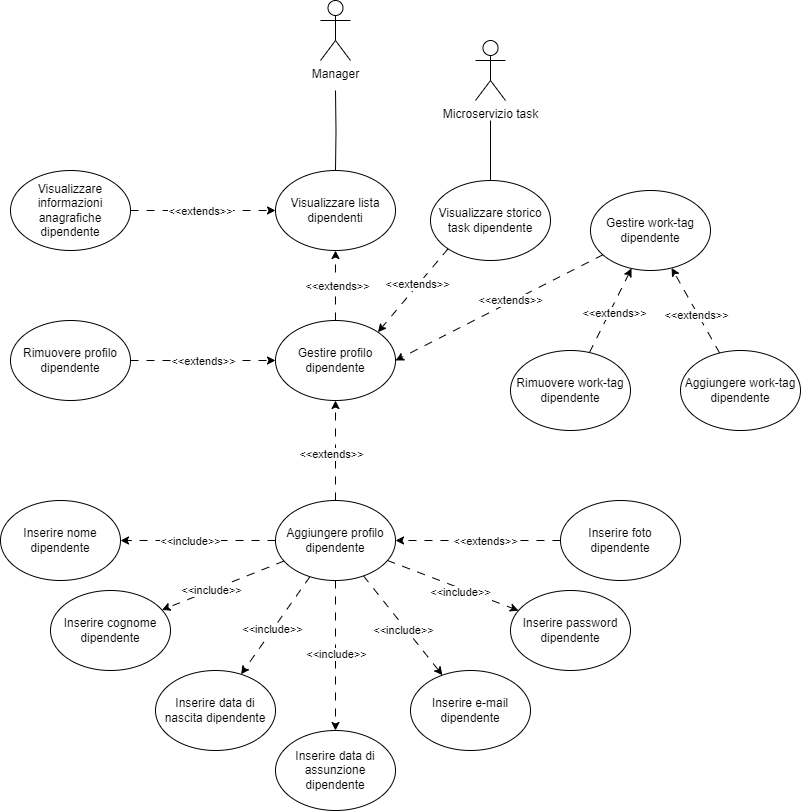
\includegraphics[width=1\textwidth]{images/UCD/RF11_gestionedipendenti_UCD.png}
	Use Case Diagram (UCD) di RF11 "Gestione Dipendenti
\end{figure}

\subsubsection*{Descrizione Use Case "Gestione Dipendenti"}
\textbf{Titolo}: Gestione Dipendenti \newline
\textbf{Riassunto}: Questo use case descrive come il manager può visualizzare e gestire i dipendenti. \newline
\textbf{Descrizione}:
\begin{enumerate}
	\item Il manager seleziona la pagina "Gestione Dipendenti";
	\item Il sito mostra la lista dei dipendenti [Exception 1];
	\item Il sito presenta un bottone in alto a destra etichettato "Aggiungi nuovo dipendente" che permette di creare un nuovo profilo inserendo i seguenti campi:
	\begin{itemize}
		\item nome[Exception 2];
		\item cognome[Exception 2]; 
		\item data di nascita[Exception 2];
		\item data di assunzione[Exception 2];
		\item e-mail[Exception 2];
		\item password[Exception 2];
		\item foto (( facoltativo ));
	\end{itemize}
	\item Il sito presenta un bottone accanto ad ogni dipendente etichettato "Rimuovi" che permette di eliminare quel profilo dipendente;
	\item Il sito presenta un bottone accanto ad ogni dipendente etichettato "Gestisci work-tag" che permette di visualizzare la lista di work-tag assegnati a quel dipendente [Exception 3], inoltre permette di:
	\begin{itemize}
		\item Aggiungere un nuovo work-tag;
		\item Rimuovere un work-tag;;
	\end{itemize}
	
\end{enumerate}
\textbf{Exceptions}
\begin{itemize}
	\item {[Exception 1]}: Se non vi sono dipendenti presenti nel sistema l'elenco sarà vuoto;
	\item {[Exception 2]}: Se il manager non ha compilato i campi "nome","cognome","data di nascita", "data di assunzione", "e-mail","password" non può creare il nuovo profilo dipendente;
	\item {[Exception 3]}: Se il dipendente non ha nessun work-tag assegnato la lista risulterà essere vuota;
\end{itemize}

\pagebreak

\section{Requisiti Non Funzionali}
Nel seguente capitolo vengono riportati i requisiti non funzionali (RNF) del sistema utilizzando tabelle strutturate e specificando misure facilmente misurabili.


\subsection*{RNF1 Intuitività e Accessibilità}
% table
\begin{center} % center the table
	\centering
	\begin{tabular}{ |p{3cm}|p{4cm}|p{4cm}|  }
		\hline
		\centering Proprietà & \qquad\quad Descrizione & \qquad\qquad Misura\\ % I found no other way...
		\hline
		Linguaggio Comprensibile & In media l’utente deve essere in grado di capire le funzionalità dell'applicazione con una
		sola lettura della descrizione. & In media, il numero di click errati che l'utente compie deve essere minore di 4. \\
		\hline
		Presenza della lingua Inglese e Italiana & Il sito presenta sia la lingua Italiana che quella Inglese, l'utente con un livello di lingua "A1" è in grado di leggere e comprendere il contenuto. & La scelta del vocabolario linguistico utilizzato è conforme con il vocabolario Italiano di livello A1 e Inglese livello A1.\\ % I found no other way...
		\hline
		Consistenza & Il sito deve avere un design consistente, utilizzando un singolo font e una palette fissa di colori. & numero di font utilizzati uguale a 1, numero di colori utilizzati minore di 6.  \\% I found no other way... 
		\hline
	\end{tabular}
\end{center}

\subsection*{RNF2 Sicurezza}
% table
\begin{center} % center the table
	\centering
	\begin{tabular}{ |p{3cm}|p{4cm}|p{4cm}|  }
		\hline
		\centering Proprietà & \qquad\quad Descrizione & \qquad\qquad Misura\\ % I found no other way...
		\hline
		Protezione dati & Il sito deve proteggere i dati sensibili utilizzando un algoritmo di hashing "SHA-3" per sarlvare e controllare le password e protocolli tls e https per ogni comunicazione tra utenti e servizi. & L'applicazione utilizza un algoritmo di hashing "SHA-3" nel salvataggio e controllo di password nel database e utilizza protocolli "tls" e "https" per ogni comunicazione tra utenti e servizi.\\
		\hline
		2 Factor Authentication (2FA) & Il sito deve verificare l'identità dell'utente attraverso il 2FA. & Impossibilità di accedere al sito senza 2FA.\\
		\hline
		Conformità password & La password di un utente deve avere una lunghezza minima di 10 caratteri e deve presentare almeno un numero,una lettera maiuscola, e un carattere speciale. &
		Numero dei caratteri maggiore di nove, presenza di almeno un numero,lettera maiuscola e carattere speciala dalla seguente lista:		\begin{verbatim} ! ? $ % ^ & * ( ) _ \end{verbatim} \begin{verbatim}- + = { [ } ] : ;\end{verbatim} \begin{verbatim}@ # | \ < , > . \end{verbatim} \\
		\hline
		
	\end{tabular}
\end{center}
\subsection*{RNF3 Privacy}
% table
\begin{center} % center the table
	\centering
	\begin{tabular}{ |p{3cm}|p{4cm}|p{4cm}|  }
		\hline
		\centering Proprietà & \qquad\quad Descrizione & \qquad\qquad Misura\\ % I found no other way...
		\hline
		GDPR & il sito deve essere conforme alle principali direttive del GDPR, tra cui il consenso esplicito per la raccolta dei dati, la trasparenza nell'uso dei dati, la possibilità di accesso e cancellazione dei dati personali da parte dell'individuo, e misure di sicurezza per proteggere tali dati. & Conforme al regolamento. \\
		\hline
	\end{tabular}
\end{center}
\subsection*{RNF4 Affidabilità e Disponibilità}
% table
\begin{center} % center the table
	\centering
	\begin{tabular}{ |p{3cm}|p{4cm}|p{4cm}|  }
		\hline
		\centering Proprietà & \qquad\quad Descrizione & \qquad\qquad Misura\\ % I found no other way...
		\hline
		Risultati desiderati & La probabilità che il sito fornisca i risultati desiderati senza interruzioni o tempi di inattività deve essere maggiore del 99\% (novantanove percento) & $\frac{\text{risultati ricevuti con successo}}{\text{risultati totali}}$ maggiore di 0.99 in media.\\ % There was no other way...
		\hline
		Operatività &  la probabilità che il sito rimanga operativo in un determinato momento
		indipendentemente dal numero di guasti già subiti dal sistema deve essere maggiore del 99\% (novantanove percento) & $ \frac{\text{secondi di attività dal lancio}}{\text{secondi totali dal lancio}}$ maggiore di 0.99 in media.\\
		\hline 
	\end{tabular}
\end{center}
\subsection*{RNF5 Performante}
% table
\begin{center} % center the table
	\centering
	\begin{tabular}{ |p{3cm}|p{4cm}|p{4cm}|  }
		\hline
		\centering Proprietà & \qquad\quad Descrizione & \qquad\qquad Misura\\ % I found no other way...
		\hline
		Aggiornamento negozio & Il sito deve elaborare l'inserimento di un articolo nel magazzino in meno di un secondo. & Il numero di secondi trascorsi da quanto viene premuto il bottone "inserisci articolo" a quando l'articolo è presente nel magazzino deve essere minore di uno. \\
		\hline 
		2 Factor Authentication (2FA)& Il sito deve inviare la mail di 2FA in meno di cinque secondi. & Secondi trascorsi da quando è stato richiesto l'invio di un coridce 2FA a quando il codice è presente nella mail minore di 5 (cinque) secondi. \\
		\hline
		Lista delle Task & Il sito deve aggiornare la lista delle task in meno di un secondo. & Il numero di secondi trascorsi per eseguire e terminare l'operazione di inserimento di una task nel database minore di 1. \\ 
		\hline

	\end{tabular}
\end{center}
\subsection*{RNF6 Compatibilità e Portabilità}
% table
\begin{center} % center the table
	\centering
	\begin{tabular}{ |p{3cm}|p{4cm}|p{4cm}|  }
		\hline
		\centering Proprietà & \qquad\quad Descrizione & \qquad\qquad Misura\\ % I found no other way...
		\hline
		Compatibilità dispositivi lato client & L'applicazione lato client  deve essere disponibile per dispositivi aventi un browser che supporta \begin{itemize}
		\item componenti html5 utilizzati
		\item https
		\item tls 1.2
		\end{itemize} &  L'applicazine ulizza https, tls 1,2 e html5.  \\
		\hline
		Compatibilità dispositivi lato server & L'applicazione lato server deve essere disponibile per computer che supportino: 
		\begin{itemize}
			\item Node js 18.18.0 LTS
		\end{itemize}
		&  L'applicazione utilizza Node js 18.18.0 LTS. \\
		\hline 
		Responsive su TV e monitor di PC e Laptop & Il sito deve potersi adattare alla dimensione degli schermi con Aspect Ratio da 4:3, 16:9, 21:9 & L'utente è in grado di eseguire correttamente ogni funzionalità dell'applicazione su schermi con aspectratio 4:3, 16:9 e 21:9. \\
		\hline
		Responsive su Smartphone & Il sito deve potersi adattare agli schermi dei seguenti Smartphone: 
		\begin{itemize}
			\item Iphone X,XR,11,\dots , 14
			\item Tutti i modelli Xiaomi dal 2018 in poi 
			\item Tutti i modelli Samsung dal 2018 in poi
			\item Tutti i modelli Motorola dal 2018 in poi 
			\item Tutti i modelli Huawei dal 2018 in poi 
		\end{itemize}
		&  L'utente è in grado di eseguire correttamente ogni funzionalità dell'applicazione sui dispositivi elencati. \\
		
		\hline
		
	\end{tabular}
\end{center}
\begin{center} % center the table
	\centering
	\begin{tabular}{ |p{3cm}|p{4cm}|p{4cm}|  }
		\hline
		Responsive su Tablet & Il sito deve potersi adattare agli schermi dei seguenti Tablet: 
		\begin{itemize}
			\item Ipad Air, Pro dal 2018 in poi
			\item Tutti i modelli Xiaomi dal 2018 in poi
			\item Tutti i modelli Samsung dal 2018 in poi
		\end{itemize} & L'utente è in grado di eseguire correttamente ogni funzionalità dell'applicazione sui dispositivi elencati. \\
		\hline
		
		
	\end{tabular}
\end{center}
\subsection*{RNF7 Mantenibilità e Scalabilità}
% table
\begin{center} % center the table
	\centering
	\begin{tabular}{ |p{3cm}|p{4cm}|p{4cm}|  }
		\hline
		\centering Proprietà & \qquad\quad Descrizione & \qquad\qquad Misura\\ % I found no other way...
		\hline
		Team di manutenzione &  Al sito deve essere affiancato, prima e dopo il rilascio ufficiale, un team di
		manutenzione che si occupi di testare ogni funzionalit`a periodicamente e
		che, su richiesta qualora ci siano problemi, sia pronto a intervenire tempestivamente
		 & E' presente un team che una volta al mese testa il sistema e le sue funzionalità, in grado di presentarsi all'azienda in meno di un giorno. \\
		\hline
		sito facilmente mantenibile & Il sito deve possedere le seguenti caratteristiche
		\begin{itemize}
			\item Il codice sorgente del back-end dev'essere modulare, utilizzando un'architetture a microserivizi
			\item Il codice sorgetne deve rispettare le linee guida del linguaggio scelto
		\end{itemize}
		& Conformità Linee guida Javascript, architettura divisa in microservizi.
		\\  \hline

	\end{tabular}
\end{center}
\subsection*{RNF8 Conformità}
\begin{center} % center the table
	\centering
	\begin{tabular}{ |p{3cm}|p{4cm}|p{4cm}|  }
		\hline
		\centering Proprietà & \qquad\quad Descrizione & \qquad\qquad Misura\\ % I found no other way...
		\hline
		Conformità leggi & L'applicazione deve essere conforme alle normative di legge in materia di siti web imposti dall'Unione Europea & Conforme ai regolamenti. \\
		\hline
		Conformità GDPR & L'applicazione deve essere conforme al GDPR, come descritto in RNF3 & Conforme ai regolamenti.\\
		\hline
		Conformità W3C WAI & L'applicazione deve essere conforme al W3C WAI (Web Accessibility Initiative) & Conforme ai regolamenti.\\ 
		\hline
	\end{tabular}

\end{center}


\chapter{Analisi del Contesto}

\section{Utenti e Sistemi Esterni}

Sono stati individuati tutti gli Utenti ed i Sistemi Esterni che fanno parte del funzionamento del sistema "Fix Mi".\\Segue una elencazione di ogni elemento con una descrizione breve adibita.


\subsection*{Utente}
Con il termine "Utente" si definisce una qualsiasi persona che abbia fatto accesso al sistema senza essersi identificati. L'Utente è in grado di:
\begin{itemize}
	\item Accedere all'area "Negozio" per visualizzare il catalogo.
	\item Accedere all'area "Informazioni / Contatti" e visualizzarne i dettagli. 
	%tutti i dettagli in esso contenuti, tra cui numeri telefonici, indirizzi di posta elettronica e posizione geografica aziendale.
\end{itemize}


\subsection*{Cliente}

Con il termine "Cliente" si intende un Utente che abbia compiuto con successo la registrazione nel sistema e che successivamente abbia fatto l'accesso nel suo profilo. Il Cliente, oltre a potere accedere a tutti i servizi offerti ad un profilo "Utente", è in grado di
\begin{itemize}
	\item Inserire gli articoli dell'area "Negozio" nel proprio carrello e, successivamente, effettuarne l'acquisto.
	\item Accedere all'area "Riparazione" per visualizzare la lista di riparazioni in corso, creare una nuova richiesta di Riparazione o eliminarne una esistente.
	%\item Inviare feedback riguardo la qualità dei servizi offerti. (Lmao non ho ancora capito se questo c'è oppure no).
\end{itemize}
\subsection*{Dipendente}

Con il termine "Dipendente" si intende quella persona che abbia stipulato un contratto di lavoro con l'azienda. Il Dipendente, oltre a poter usufruire di tutti i servizi adibiti ad un profilo Cliente, può:
\begin{itemize}
	\item Accedere all'area "Magazzino" per visualizzare la lista dei prodotti posseduti, aggiungere un nuovo articolo o rimuoverne uno esistente.
	\item Accedere all'area "Task" per visualizzare la lista delle Task, crearne una nuova, contrassegnarla o rimuoverne una esistente. 
\end{itemize}

\subsection*{Manager}

Con il termine "Manager" si intende quella persona che abbia il completo controllo del sistema e dell'azienda. Il Manager, oltre a potere accedere a tutte le aree offerte al profilo Dipendente, è in grado di:
\begin{itemize}
	\item Accedere all'area "Gestione Dipendenti" per visualizzarne la lista, aggiungere un nuovo profilo Dipendente o eliminarne uno esistente.
\end{itemize}

\subsection*{Server Mail}
Attraverso la Server Mail, il sistema è in grado di mandare e ricevere e-mail. 

\subsection*{Database}
Il database memorizza il catalogo del negozio, l'inventario del magazzino e le informazioni riguardanti i profili gestiti dal sistema (es. e-mail e password).

\subsection*{PayPal e Nexi}
I servizi esterni "PayPal" e "Nexi" permettono al Cliente di effettuare acquisti all'interno del sistema.

\subsection*{OpenStreetMap}
Il servizio esterno "OpenStreetMap" fornisce dati geografici al sistema.%per visualizzare la posizione aziendale geografica in cartina.

\subsection*{2FA}
Il 2FA ("Two Factor Authentication") si occupa di verificare che la e-mail inserita dall'utente in procinto di registrarsi o accedere sia corretta ed esistente.
%In particolare il codice contenuto nel 2FA viene spedito all'indirizzo di posta elettronica inserito dall'Utente che, nel caso sia inesistente, non potrebbe essere visualizzato. (Non sono sicuro se scrivere anche questo o no....)

\subsection*{Microservizi}
Autentication Server, Microservizio Task


\section{Diagramma di Contesto}

Spiegare la back-end andando su vari livelli di dettaglio:
\begin{itemize}
	\item Context diagram generale
	\item Divisione in processi
	\item Divisione in Sub Processi
	\item Data flow diagram per i processi (e i sub processi se siamo bravi)
\end{itemize}
\chapter{Analisi dei Componenti}

\section{Definizione dei Componenti}

Componenti interni della mia applicazione e come interagiscono\\
Sostanzialmente sono i componenti usati nei RF in questo documento

\subsection*{Autenticazione}
\textbf{Descrizione: } Questa componente corrisponde al microservizio Autenticazione. Si occupa del controllo dell'accesso ai servizi dell'applicazione da parte degli utenti,
e fornisce i dati di autenticazione e di anagrafica degli utenti agli altri componenti che li richiedono.

\uline{\textit{Interfaccia richiesta - Token utente: }}La componente richiede al database il token di un utente
\\ \\ \uline{\textit{Interfaccia fornita - Token utente: }}La componente fornisce il token di un determinato utente alle componenti che lo richiedono
\\ \\ \uline{\textit{Interfaccia fornita - Verifica token utente: }}La componente verifica l'esistenza di un determinato utente su richiesta di altre componenti, comunicando anche il ruolo di quel determinato utente
\\ \\ \uline{\textit{Interfaccia richiesta - Dati personali utente: }} La componente richiede al database i dati personali di un determinato utente, quali:
\begin{itemize}
	\item username
	\item email
	\item ruolo (cliente, dipendente o manager)
	\item nazionalità
\end{itemize}  
Possono essere richiesti tutti i dati o solo alcuni
\\ \\ \uline{\textit{Interfaccia fornita - Verifica credenziali: }}La componente verifica che le credenziali di un utente fornite siano corrette 
\\ \\ \uline{\textit{Interfaccia fornita - Nuovo utente: }}La componente riceve i dati per la creazione di un nuovo utente. I dati sono i seguenti:
\begin{itemize}
	\item username
	\item email
	\item password
	\item ruolo (cliente dipendente o manager)
	\item nazionalità
\end{itemize}
\uline{\textit{Interfaccia richiesta - Nuovo utente: }}La componente fornisce al database i seguenti dati per la creazione di un nuovo utente.
\begin{itemize}
	\item username
	\item email
	\item password hash
	\item ruolo (cliente, dipendente o manager)
	\item nazionalità
\end{itemize}
\uline{\textit{Interfaccia fornita - Verifica esistenza email: }} La componente verifica se la mail appartiene già a un utente del sistema
Di questo componente fanno parte due sub-componenti, Login e Registrazione, descritte di seguito.
\subsection*{Login}
\textbf{Descrizione: }Questa componente si occupa del processo di login, descritto in RF1
\\ \\ \uline{\textit{Interfaccia richiesta - Email e password: }} Viene richiesta l'email e la password all'utente che vuole autenticarsi
\\ \\ \uline{\textit{Interfaccia richiesta - Verifica credenziali }}La componente richiede la verifica delle credenziali da parte della componente Autenticazione
\\ \\ \uline{\textit{Interfaccia richiesta - Invio Codice 2FA}} La componente fornisce alla componente "Server mail" il codice 2 Factor Authentication da inviare all'utente
\uline{\textit{Interfaccia richiesta - Controllo 2FA }} Viene richiesto all'utente l'inserimento del codice 2 Factor Authentication ricevuto tramite mail
\\ \\ \uline{\textit{Interfaccia richiesta - Token utente}} Viene richiesto alla componente "Autenticazione" il token dell'utente appena autenticato
\\ \\ \uline{\textit{Interfaccia fornita - Token utente}} Viene fornito all'utente il proprio token

\subsection*{Cambio password}
\textbf{Descrizione: }Questa componente si occupa del processo di cambio password, descritto in RF1
\\ \\ \uline{\textit{Interfaccia richiesta - Email: }} Viene richiesta all'utente che vuole cambiare password la propria mail
\\ \\ \uline{\textit{Interfaccia richiesta - Verifica esistenza email}}: La componente richiede alla componente "Autenticazione" l'esistenza di un profilo utente con la email fornita.
\\ \\ \uline{\textit{Interfaccia richiesta - Invio Codice 2FA: }} La componente fornisce alla componente "Server mail" Il codice 2 Factor Authentication da inviare all'utente
\\ \\ \uline{\textit{Interfaccia richiesta - 2FA: }} Viene richiesto all'utente l'inserimento del codice 2 Factor Authentication appena ricevuto
\\ \\ \uline{\textit{Interfaccia richiesta - Nuova password}} Viene richiesto all'utente l'inserimento della nuova password due volte
\\ \\ \uline{\textit{Interfaccia fornita - Nuova password}} Viene fornita la nuova password al database, che procede ad aggiornarla

\subsection*{Registrazione}
\textbf{Descrizione: } Questa componente si occupa del processo di registrazione, descritto in RF2
\\ \\ \uline{\textit{Interfaccia richiesta - Dati registrazione utente: }}Per registrarsi, vengono richiesti all'ospite i seguenti dati
\begin{itemize}
	\item email
	\item password
	\item conferma password
	\item username
	\item nazionalità
\end{itemize}
\uline{\textit{Interfaccia richiesta - Verifica esistenza email: }}La componente richiede alla componente "Autenticazione" l'esistenza di un utente con la mail fornita,
per decidere se procedere o meno con la registrazione
\\ \\ \uline{\textit{Interfaccia richiesta - Invio Codice 2FA: }} La componente fornisce Il codice 2 Factor Authentication alla componente "Server mail", da inviare all'ospite che vuole registrarsi
\\ \\ \uline{\textit{Interfaccia richiesta - Controllo 2FA: }} La componente richiede all'ospite il codice 2FA appena ricevuto tramite mail
\\ \\ \uline{\textit{Interfaccia fornita - Nuovo utente}} Vengono forniti i dati della registrazione dell'utente al componente "Autenticazione", con il ruolo "cliente"
\\ \\ \uline{\textit{Interfaccia richiesta - Token utente}} Viene richiesto alla componente "Autenticazione" il token dell'utente appena registrato
\\ \\ \uline{\textit{Interfaccia fornita - Token utente}} Viene fornito all'utente il proprio token

\subsection*{Server mail}
\textbf{Descrizione}: Questa componente si occupa dell'invio delle e-mail 2FA \\
\uline{\textit{Interfaccia fornita - Invio Codice 2FA}}:
La componente fornisce la possibilità di inviare una mail con un codice 2FA all'email di un determinato utente.
\subsection*{Negozio}

\textbf{Descrizione}: Questa componente si occupa di mostrare  ed interagire con il negozio ad ogni tipo di utente in base al livello di privilegi dello stesso. In particolare permette di ricercare un articolo nel negozio, ordinarlo in ordine alfabetico e permettere di aggiungere un prodotto al carrello.
\\
\\
\uline{\textit{Interfaccia Richiesta - Lista Articoli.}} Il Negozio si aspetta di ricevere la lista degli articoli presenti nel magazzino per poterli mostrare, ossia il nome dell'articolo, una foto e una descrizione. \\ \\
\uline{\textit{Interfaccia Richiesta - Cerca Articoli}}
Il Negozio può visualizzare la lista degli articoli presenti nel magazzino tali che il nome contiene una stringa di ricerca.
\uline{\textit{Interfaccia Richiesta - Aggiungi al Carrello.}} Tramite il negozio si può aggiungere un elemento al carrello prima di poterlo acquistare. \\ \\
\uline{\textit{Interfaccia Richiesta - Token Utente.}} Il Negozio utilizzerà il token utente per verificare il livello di privilegio dell'utente.

\subsection*{Carrello}

\textbf{Descrizione}: Questa componente registra l'inserimento e la rimozione degli articoli nel carrello e permette di effettuare l'acquisto di tali articoli. \\ \\
\uline{\textit{Interfaccia Fornita - Aggiungi al Carrello.}} Il carrello permette al Negozio di poter aggiungere articoli e salvarli nel carrello.\\ \\
\uline{\textit{Interfaccia Richiesta - Aggiungi Articolo.}} Il Carrello si interfaccia con un database per il salvataggio degli articoli nel carrello oltre la sessione.\\ \\
\uline{\textit{Interfaccia Richiesta - Rimozione Articolo.}} 
Il Carrello si interfaccia con un database per rimuovere un articolo dal carrello in modo permanente.\\ \\
\uline{\textit{Interfaccia Richiesta - Svuota Carrello.}}
Il Carrello si interfaccia con un database per svuotare tutti i dati degli articoli presenti nel carrello in modo permanente.\\ \\
\uline{\textit{Interfaccia Richiesta - Token Utente.}} Il carrello utilizzerà il token utente per verificare il livello di privilegio dell'utente.\\ \\1
\uline{\textit{Interfaccia Richiesta - Pagamento}}
Il Carrello si interfaccia con un sistema esterno per effettuare il pagamento degli articoli salvati nel carrello.

\subsection*{Home}
% Non so se assistenza, feedback e riparazione vanno qua dentro
\subsection*{Riparazione}
\textbf{Descrizione}: Questa componente si occupa di prendere le richieste di riparazione degli utenti e di mostrare quelle già richieste
\uline{\textit{Interfaccia Richiesta - Token utente}}: 
Viene richiesto all'utente il proprio token identificativo\\
\uline{\textit{Interfaccia Richiesta - Verifica token utente}}:
La componente richiede la verifica del token utente alla componente "Autenticazione"\\
\uline{\textit{Interfaccia Richiesta - Nuova riparazione}}:
La componente richiede all'utente le informazioni riguardanti la richiesta di riparazione:
\begin{itemize}
	\item telefono
	\item email
	\item cognome
	\item nome
	\item descrizione
	\item foto(opzionale)
\end{itemize}
\uline{\textit{Interfaccia richiesta - Creazione task}}: 
La componente richiede alla componente "Task" la creazione di una nuova task riparazione con i dettagli inseriti dall'utente\\
\uline{\textit{Interfaccia fornita - Lista riparazioni}}: 
La componente fornisce all'utente la lista delle riparazioni che ha richiesto in precedenza\\
\uline{\textit{Interfaccia richiesta -Lista task riparazione}}: 
La componente richiede alla componente "Task" la lista delle riparazioni richieste dall'utente in precedenza

\subsection*{Assistenza}:
Questa componente si occupa di raccogliere le richieste di assistenza degli utenti
\uline{\textit{Interfaccia Richiesta - Token utente}}: 
Viene richiesto all'utente il proprio token identificativo\\
\uline{\textit{Interfaccia Richiesta - Verifica token utente}}:
La componente richiede la verifica del token utente alla componente "Autenticazione"\\
\uline{\textit{Interfaccia Richiesta - Richiesta assistenza}}:
La componente richiede all'utente le informazioni riguardanti la propria richiesta di assistenza:
\begin{itemize}
	\item descrizione
	\item e-mail
\end{itemize}
\uline{\textit{Interfaccia Richiesta - Creazione task}}:
La componente richiede alla componente "Task" la creazione di una nuova task "assistenza" con i dettagli inseriti dall'utente

\subsection*{Feedback}:
Questa componente si occupa di raccogliere i feedback degli utenti
\uline{\textit{Interfaccia Richiesta - Token utente}}: 
Viene richiesto all'utente il proprio token identificativo\\
\uline{\textit{Interfaccia Richiesta - Verifica token utente}}:
La componente richiede la verifica del token utente alla componente "Autenticazione"\\
\uline{\textit{Interfaccia Richiesta - Invia feedback}}:
La componente richiede all'utente le informazioni riguardanti il feedback che desidera inviare:
\begin{itemize}
	\item disponibilità azienda
	\item velocità riparazione
	\item soddisfazione riparazione
	\item soddisfazione sito web
	\item idee per migliorare
\end{itemize}
\uline{\textit{Interfaccia Richiesta - Creazione Task}}:
La componente richiede alla componente "Task" la creazione di una nuova task "assistenza" con i dettagli inseriti dall'utente

\subsection*{Magazzino}
\textbf{Descrizione: } Questa componente permette il salvataggio e rimozione degli articoli in un database esterno.\\ \\
\uline{\textit{Interfaccia Fortnita - Aggiungi Articolo}}
Il Magazzino permette l'aggiunta di un articolo per essere salvato per un periodo prolungato.\\ \\
\uline{\textit{Interfaccia Fornita - Rimuovi Articolo}}
Il Magazzino permette la rimozione di un articolo dallo stesso.\\ \\
\uline{\textit{Interfaccia Fornita - Lista Articoli}}
Il Magazzino permette ad altre componenti di aver accesso a tutti articoli presenti, inoltre la lista può essere inviata in senso alfabetico crescente o descrescente.\\ \\
\uline{\textit{interfaccia Fornita - Cerca Articoli}}
Il Magazzino permette di ricercare gli articoli che contengono una certa stringa.\\ \\
\uline{\textit{Interfaccia Richiesta - Token Utente.}} Il Magazzino utilizzerà il token utente per verificare il livello di privilegio dell'utente.\\ \\
\uline{\textit{Interfaccia Richiesta - Aggiungi Elemento}}
Il Magazzino si interfaccia con un database esterno per il salvataggio degli articoli.\\ \\
\uline{\textit{Interfaccia Richiesta - Rimuovi Elemento}}
Il Magazzino si interfaccia con un database esterno per la rimozione permanente di un articolo.\\ \\
\uline{\textit{Interfaccia Richiesta - Lista Articoli}}
Il Magazzino si interfaccia con un database esterno per ottenere una lista degli articoli salvati del database.\\ \\
\uline{\textit{Interfaccia Richiesta - Cerca element}}
Il Magazzino si interfaccia con un database esterno per cercare gli articoli che contengono una stringa nel nome.\\ \\

\subsection*{Task}

\textbf{Descrizione}: Questa componente si occupa di gestire il sistema task della applicazione.\\\\
\uline{\textit{Interfaccia Richiesta - Token Utente}}:
La componente richiede al dipendente(o manager) il proprio token utente \\ \\
\uline{\textit{Interfaccia Richiesta - Verifica token utente}}: 
La componente richiede la verifica del token utente alla componente "Autenticazione", per verificare se ha il ruolo adeguato per poter accedere \\ \\ 
\uline{\textit{Interfaccia Richiesta - work-tag dipendente}}: 
La componente richiede al database le work-tag di un determinato dipendente \\ \\
\uline{\textit{Interfaccia Fornita - work-tag dipendente}}: 
la componente fornisce le work-tag di un dipendente alle componenti che lo richiedono\\ \\
\uline{\textit{Interfaccia Fornita - Aggiunta work-tag dipendente}}: 
La componente fornisce la possibilità di aggiungere work-tag per un determinato dipendente alle componenti che lo richiedono.\\ \\
\uline{\textit{Interfaccia Richiesta - Aggiunta work-tag dipendente}}: 
La componente richiede al database di inserire una work-tag per un determinato dipendente\\ \\ 
\uline{\textit{Interfaccia Fornita - Rimozione work-tag dipendente}}: 
La componente fornisce la possibilità di rimuovere work-tag per un determinato dipendente alle componenti che lo richiedono.\\ \\ 
\uline{\textit{Interfaccia Richiesta - Rimozione work-tag dipendente}}:  
La componente richiede al database di rimuovere una work-tag per un determinato dipendente \\ \\ 
\uline{\textit{Interfaccia Richiesta - Creazione task}}:
La componente richiede al database di creare una task \\\\
\uline{\textit{Interfaccia Fornita - Creazione task}}: 
La componente fornisce la possibilità di creare una task da parte delle componenti che lo richiedono \\\\
\uline{\textit{Interfaccia richiesta - Lista task in lavorazione}}: 
La componente richiede al database la lista delle task in lavorazione, filtrata in base a vari filtri\\\\
\uline{\textit{Interfaccia fornita - Lista task in lavorazione}}: 
La componente permette al dipendente di vedere  la lista delle task in lavorazione\\\\
\uline{\textit{Interfaccia richiesta - Lista task in pausa/da eseguire}}: 
La componente richiede al database la lista delle task in pausa/da eseguire, filtrata in base a vari filtri\\\\
\uline{\textit{Interfaccia fornita - Lista task in pausa/da eseguire}}: 
La componente permette al dipendente di vedere la lista delle task che può eseguire\\\\
\uline{\textit{Interfaccia fornita - Scelta task}}: 
La componente permette al dipendente di scegliere una task da eseguire\\\\
\uline{\textit{Interfaccia richiesta - modifica stato task}}:
 La componente richiede al database di modificare lo stato di una task\\\\
\uline{\textit{Interfaccia fornita - modifica stato task}}: 
La componente permette al dipendente di modificare lo stato della task scelta\\\\
\uline{\textit{Interfaccia fornita - Lista task riparazione}}:
La componente permette alla componente "Riparazione" di richiedere la lista delle riparazioni richieste da un determinato cliente\\\\
\uline{\textit{Interfaccia fornita - Storico task dipendente}}:
La componente permette alla componente "Gestione Dipendenti" di richiedere la lista delle task svolte/in svolgimento di un determinato dipendente




\subsection*{Gestione Dipendenti}
\textbf{Descrizione}: Questa componente si occupa della gestione dei profili dei dipendenti, della loro creazione,modifica e eliminazione.\\\\
\uline{\textit{Interfaccia Richiesta - Token Utente}}:
La componente richiede al manager il proprio token utente \\ \\
\uline{\textit{Interfaccia Richiesta - Verifica token utente}}: 
La componente richiede la verifica del token utente alla componente "Autenticazione", per verificare se ha il ruolo adeguato per poter accedere \\ \\ 
\uline{\textit{Interfaccia Richiesta - Lista dipendenti}}:
La componente richiede al database la lista dei dipendenti e le corrispettive informazioni anagrafiche\\\\
\uline{\textit{Interfaccia Fornita - Lista dipendenti}}:
La componente fornisce al manager la lista dei dipendenti\\\\
\uline{\textit{Interfaccia Fornita - Informazioni dipendente}}:
La componente fornisce al manager le informazioni di un determinato dipendente\\\\
\uline{\textit{Interfaccia Fornita - Rimuovere profilo}}:
La componente fornisce al manager la possibilità di rimuovere un profilo dipendente\\\\
\uline{\textit{Interfaccia Richiesta - Rimuovere profilo}}:
La componente richiede al database la rimozione di un profilo dipendente dal database\\\\
\uline{\textit{Interfaccia Fornita - Aggiungere profilo}}:
La componente fornisce al manager la possibilità di aggiungere un nuovo profilo dipendente inserendo i seguenti parametri:
\begin{itemize}
	\item nome dipendente
	\item cognome dipendente
	\item data di nascita
	\item data di assunzione
	\item email 
	\item password
	\item foto(opzionale)
\end{itemize}
\uline{\textit{Interfaccia Richiesta - Nuovo utente}}: 
La componente richiede alla componente "Registrazione" la creazione di un nuovo utente con il ruolo "dipendente"\\\\
\uline{\textit{Interfaccia Richiesta - Aggiungere profilo}}:
La componente richiede al database l'aggiunta di un nuovo profilo dipendente\\\\
\uline{\textit{Interfaccia Richiesta -Aggiunta work-tag dipendente}}:
La componente richiede alla componente "Task" l'aggiunta di una work-tag al profilo di un determinato dipendente\\\\
\uline{\textit{Interfaccia Fornita - Aggiunta work-tag dipendente}}:
La componente fornisce al manager la possibilità di aggiungere una work-tag a un determinato dipendente.\\\\
\uline{\textit{Interfaccia Richiesta - Rimozione work-tag dipendente}}:
La componente richiede alla componente "Task" l'aggiunta di una work-tag al profilo di un determinato dipendente\\\\
\uline{\textit{Interfaccia Fornita - Rimozione work-tag dipendente}}:
La componente fornisce al manager la possibilità di eliminare una work-tag di un determinato dipendente.\\\\
\uline{\textit{Interfaccia richiesta - Storico task dipendente}}:
La componente richiede alla componente "Task" lo storico delle task di un determinato dipendente.\\\\
\uline{\textit{Interfaccia fornita - Storico task dipendente}}:
La componente fornisce al manager la possibilità di visualizzare lo storico delle task di un determinato dipendente

% \subsection{Database} ?
\subsection{Database}


\section{Diagramma dei Componenti}

\end{document}